%!TEX root = ../../thesis.tex
\section{Components}

The implementation of XBMCMagic was an experiment to write as less JavaScript code as possible and to use AngularJS's expressions wherever it was possible. Most frontend code has been achieved by solely using expressions, built-in directives and lean controllers which mostly act as glue code to services or third party libraries.

\subsection{Controllers}

\begin{figure}[htb]
  \centerline{
    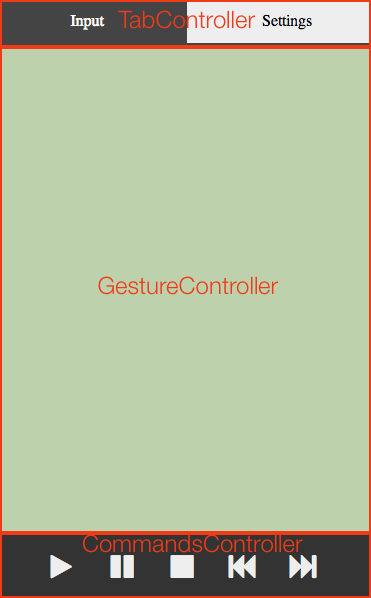
\includegraphics[width=0.4\linewidth]{images/xbmc-magic-screen-1.png}
    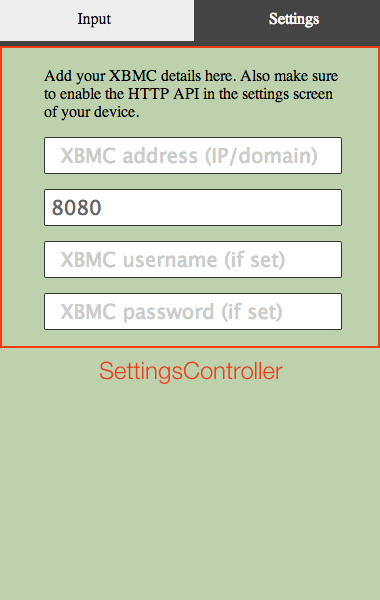
\includegraphics[width=0.41\linewidth]{images/xbmc-magic-screen-2.png}
  }
  \caption[left: initial screen, right: settings screen]{left: initial screen, right: settings screen}
  \label{fig:xbmcmagic-controllers}
\end{figure}

The app consists of only four controllers which are shown in \reffigure{fig:xbmcmagic-controllers}:

\subsubsection{TabController}

The TabController takes care of switching the currently visible tab and consists only of expressions in the template and one line of JavaScript in the controller file itself (\code{\$scope.currentTab = 0}). The controller is registered in the first line of \reflisting{lst:tab-controller} and from then on the logic relies entirely on directives and expressions. Line 9 switches (\code{ng-switch}) the shown content tab based on the value of \code{currentTab}, which is changed on click (\code{ng-click}) on one of the tab headers in line 3 or in line 6. Furthermore, the visual state of a tab header is changed according to the state of \code{currentTab} as well by using the \code{ng-class} directive.

\begin{lstlisting}[language=HTML, caption=TabController expressions, label=lst:tab-controller]
  <div class="tabs" ng-controller="TabController">
    <div class="tab-header">
        <div  ng-class="{`active': currentTab == 0}"
              ng-click="currentTab = 0">Input</div>

        <div  ng-class="{`active': currentTab == 1}"
              ng-click="currentTab = 1">Settings</div>
    </div>
    <div ng-switch="currentTab">
      <div ng-switch-when="0"><!-- GESTURES --></div>
      <div ng-switch-when="1"><!-- SETTINGS --></div>
    </div>
  </div>
\end{lstlisting}

\subsubsection{GestureController}

The GestureController detects and interprets the user's swipe gestures. For this purpose it uses Hammer.js\footnote{\url{https://github.com/EightMedia/hammer.js}, last-checked on 22/04/2014}, a gesture-detection library, and the \code{xbmcRemote} service(see \refchapter{subsubsec:xbmcRemote}).

\begin{lstlisting}[language=JavaScript, caption=GestureController mappings, label=lst:gesture-controller]
  hammeredGestureTarget.on('swipeup', function() {
    xbmcRemote.up();
  });
\end{lstlisting}

\reflisting{lst:gesture-controller} \ demonstrates the binding between the \code{hammeredGestureTarget} (a hammer.js target) and the \code{xbmcRemote} service object. Each gesture is associated with one specific action. In this case, a \code{swipeup} would execute the \code{up} command in the XBMC media center, which is used for navigating between elements. Simple swipes e.g. are always used for visual navigation. Another example for gestures is the double tap, it executes the `back' command and navigates to the previous dialog.

\subsubsection{CommandsController}

The CommandsController is similar to the GestureController and only acts as a connection between \code{xbmcRemote} and the user interface. Instead of using gestures, the buttons use \code{ng-click} to execute the actions. The buttons only act as shortcuts to functionalities that could also be executed by combining some gestures and navigating visually.

\subsubsection{SettingsController}

Before the remote control can be used, it is essential to add the network information for the desired XBMC media center. The SettingsController provides an easy form to type in all required details that are needed to connect to the server. It makes use of the values that are provided by the \code{xbmcSettings} service (see \refchapter{subsubsec:xbmcSettings}). Again, the controller only uses built-in directives (\code{ng-change} and \code{ng-model}, see \reflisting{lst:settings-controller}) and provides a simple \code{save} method that points to the \code{xbmcSettings} service.

\begin{lstlisting}[language=HTML, caption=SettingsController bindings, label=lst:settings-controller]
  <form ng-change="save()">
    <input type="text" ng-model="settings.address"/>
  </form>
\end{lstlisting}

\subsection{Services}

\subsubsection{xbmcRemote}
\label{subsubsec:xbmcRemote}

The XBMC media center provides a JSON-RPC\footnote{\url{http://www.jsonrpc.org/specification}, last-checked on 23/04/2014} API\footnote{\url{http://wiki.xbmc.org/?title=JSON-RPC_API}, last-checked on 23/04/2014} which can be used to control the interface. It gives third-party applications complete control over the user interface and it provides access to metadata about the currently selected or the playing media stream. The \code{xbmcRemote} service provides a simple way to send actions to the media center by completely hiding the connection logic and providing a simplified API to the controllers that need to send actions. At its core, the service uses AngularJS's \code{\$http} service to prepare and to send messages. In addition, it uses the connection information, which is provided by the \code{xbmcSettings} service.

\subsubsection{xbmcSettings}
\label{subsubsec:xbmcSettings}

The connection settings are saved using the device's \code{localStorage}, a simple key-value storage that is available in all targeted mobile web browsers\footnote{\url{http://caniuse.com/namevalue-storage}, last-checked on 23/04/2014}. Therefore, the \code{xbmcSettings} service acts as a central interaction point that automatically loads the configuration when the application starts. It furthermore provides an API to persist the current configuration which is used by the \code{SettingsController} when a form change is detected.